\documentclass[final]{article}
\usepackage{multicol}    % For multiple columns
\usepackage{graphicx}     % For images
\usepackage{amsmath, amssymb} %for math
\usepackage{mathptmx} % Times fonts with scalable math
\usepackage{lmodern}    %font type
\usepackage[T1]{fontenc} % For better encoding
\usepackage{color}        % Color support
\usepackage[utf8]{inputenc} % UTF-8 encoding
\usepackage{enumitem}     % Custom list formatting
\usepackage[paperwidth=48in,paperheight=36in,margin=1in]{geometry} % Custom size
\usepackage{tikz}         % For positioning elements

\usepackage{cite}         % For citation management
\usepackage{float}
\usepackage{array}
\usepackage{natbib}


% Custom Colors (Adjust based on poster needs)
\definecolor{DarkBlue}{rgb}{0.1,0.2,0.6}

% Title Formatting (Use large manual font sizes)
\newcommand{\posterTitle}[1]{
    \noindent{
        \color{DarkBlue}
        \fontsize{72}{80}\bfseries #1
    }
}

% Author and Institution Formatting
\newcommand{\posterAuthors}[1]{
    \noindent{
        \color{black}
        \fontsize{40}{48}\bfseries #1
    }
}

% Section Heading
\newcommand{\posterSection}[1]{
    \noindent{
        \color{DarkBlue}
        \fontsize{50}{60}\bfseries #1
    }
    \vspace{0.5em}
    \hrule
    \vspace{1em}
}

% Regular Body Text
\renewcommand{\normalsize}{\fontsize{28}{34}\selectfont}

%Bold text
\newcommand{\boldtext}[1]{{\fontseries{b}\selectfont #1}}

% Begin Document
\begin{document}

% Navy Blue Bar with Title, Authors, and Logo
\begin{tikzpicture}[remember picture, overlay]
    % Draw the navy-blue rectangle bar
    \fill[DarkBlue] (current page.north west) rectangle ++(48in, -3.5in); % Adjust width and height as needed

    % Add Title in the bar
    \node[anchor=north, yshift=-0.5in, xshift=1cm] at (current page.north) {
    \color{white}
    \fontsize{72}{80}\bfseries
    MRI SAFETY AND RETAINED EPICARDIAL LEADS
};

    % Add Author Name below the Title
    \node[anchor=north, yshift=-1.8in] at (current page.north) {
    \color{white}
    \fontsize{50}{58}\bfseries
    \parbox{\textwidth}{ % Adjust the width as needed
        \centering % To center the text
        \textbf{Daniel Juarez} \\ %, Author2 Bold name with a line break
        Department of Physics, Creighton University, Omaha, NE
    }
};

    % Add University Logo in the bar
    %\node[anchor=north east, xshift=-1cm, yshift=-1cm] at (current page.north east) {
  %  \includegraphics[width=3in]{university-logo.png}
%};

\end{tikzpicture}

% Add vertical dividers between columns
\begin{tikzpicture}[remember picture, overlay]
    % Divider 1
    \draw[DarkBlue, thick] (15.2in, 0) -- (15.2in, -34in); % Adjusted to align within the text
    % Divider 2
    \draw[DarkBlue, thick] (30.5in, 0) -- (30.5in, -34in); % Divider for the second column
\end{tikzpicture}


\vspace{1.8in} % Add appropriate spacing to move the content down

% Begin Multicolumn Layout
\begin{multicols}{3}

% Introduction Section
\posterSection{Introduction}
%What’s the problem?
There is a concern on whether a patient with retained post-surgical epicardial leads can safely be scanned in an MRI device because the interaction of the magnetic field, RF and gradients with these leads are still not well defined. They may rise problems such as RF-induced heating, translational forces, and torques and induced currents. In previous graduate student thesis and research, these risks and issues were highlighted.  \cite{haddix2022, aboyewa2021}. The thesis pointed out that over 50\% of patients with cardiac implantable electronic devices (CIEDs) will require MRI in their lifetime \cite{aboyewa2021}. Moreover, there is a lack of consensus across clinical guidelines that leaves physicians with the task to assess risks on a case-by-case basis.

\boldtext{Objective:} To synthesize findings on MRI safety with epicardial leads, focusing on RF heating, magnetic forces, and torques, while identifying research gaps and proposing strategies for safer imaging.

\vspace{1cm}

% Risks Section
\posterSection{Risks of MRI with Epicardial Leads}
%Why does it matter?
\begin{itemize}
    \item \textbf{RF-Induced Heating:} Leads can act as antennas, they absorb RF energy and cause localized tissue heating, particularly at the lead tips \cite{aboyewa2021}.
    \item \textbf{Translational Forces:} The strong magnetic field can induce translational forces, pulling ferromagnetic materials toward the scanner's isocenter. These forces depend on lead material and length. \cite{haddix2022}.
    \item \textbf{Torque:} Leads experience twisting forces that align them with the magnetic field, this can cause discomfort or tissue damage if the lead length is significant \cite{haddix2022}.
    \item \textbf{Electrical Stimulation:} RF fields can induce currents in leads and stimulate cardiac tissue. This remains an underexplored area requiring further research \cite{aboyewa2021}.
    \item \textbf{Device Malfunction:} MRI fields may interfere with pacemaker settings, causing unintended pacing or disabling the device altogether \cite{aboyewa2021}.
\end{itemize}

% Backgorund Section
\posterSection{Background}
%How was it studied?
To answer whether safety concerns signify the outlined risk tissue-equivalent phantoms were designed, created and tested in previous research. Figure \ref{fig:phantom_design} shows the the phantom design and experimental setup used and table \ref{tab:phantom_characterization} compares the properties of the phantom materials to ASTM standards, confirming their clinical relevance.

\begin{figure}[H]
    \centering
    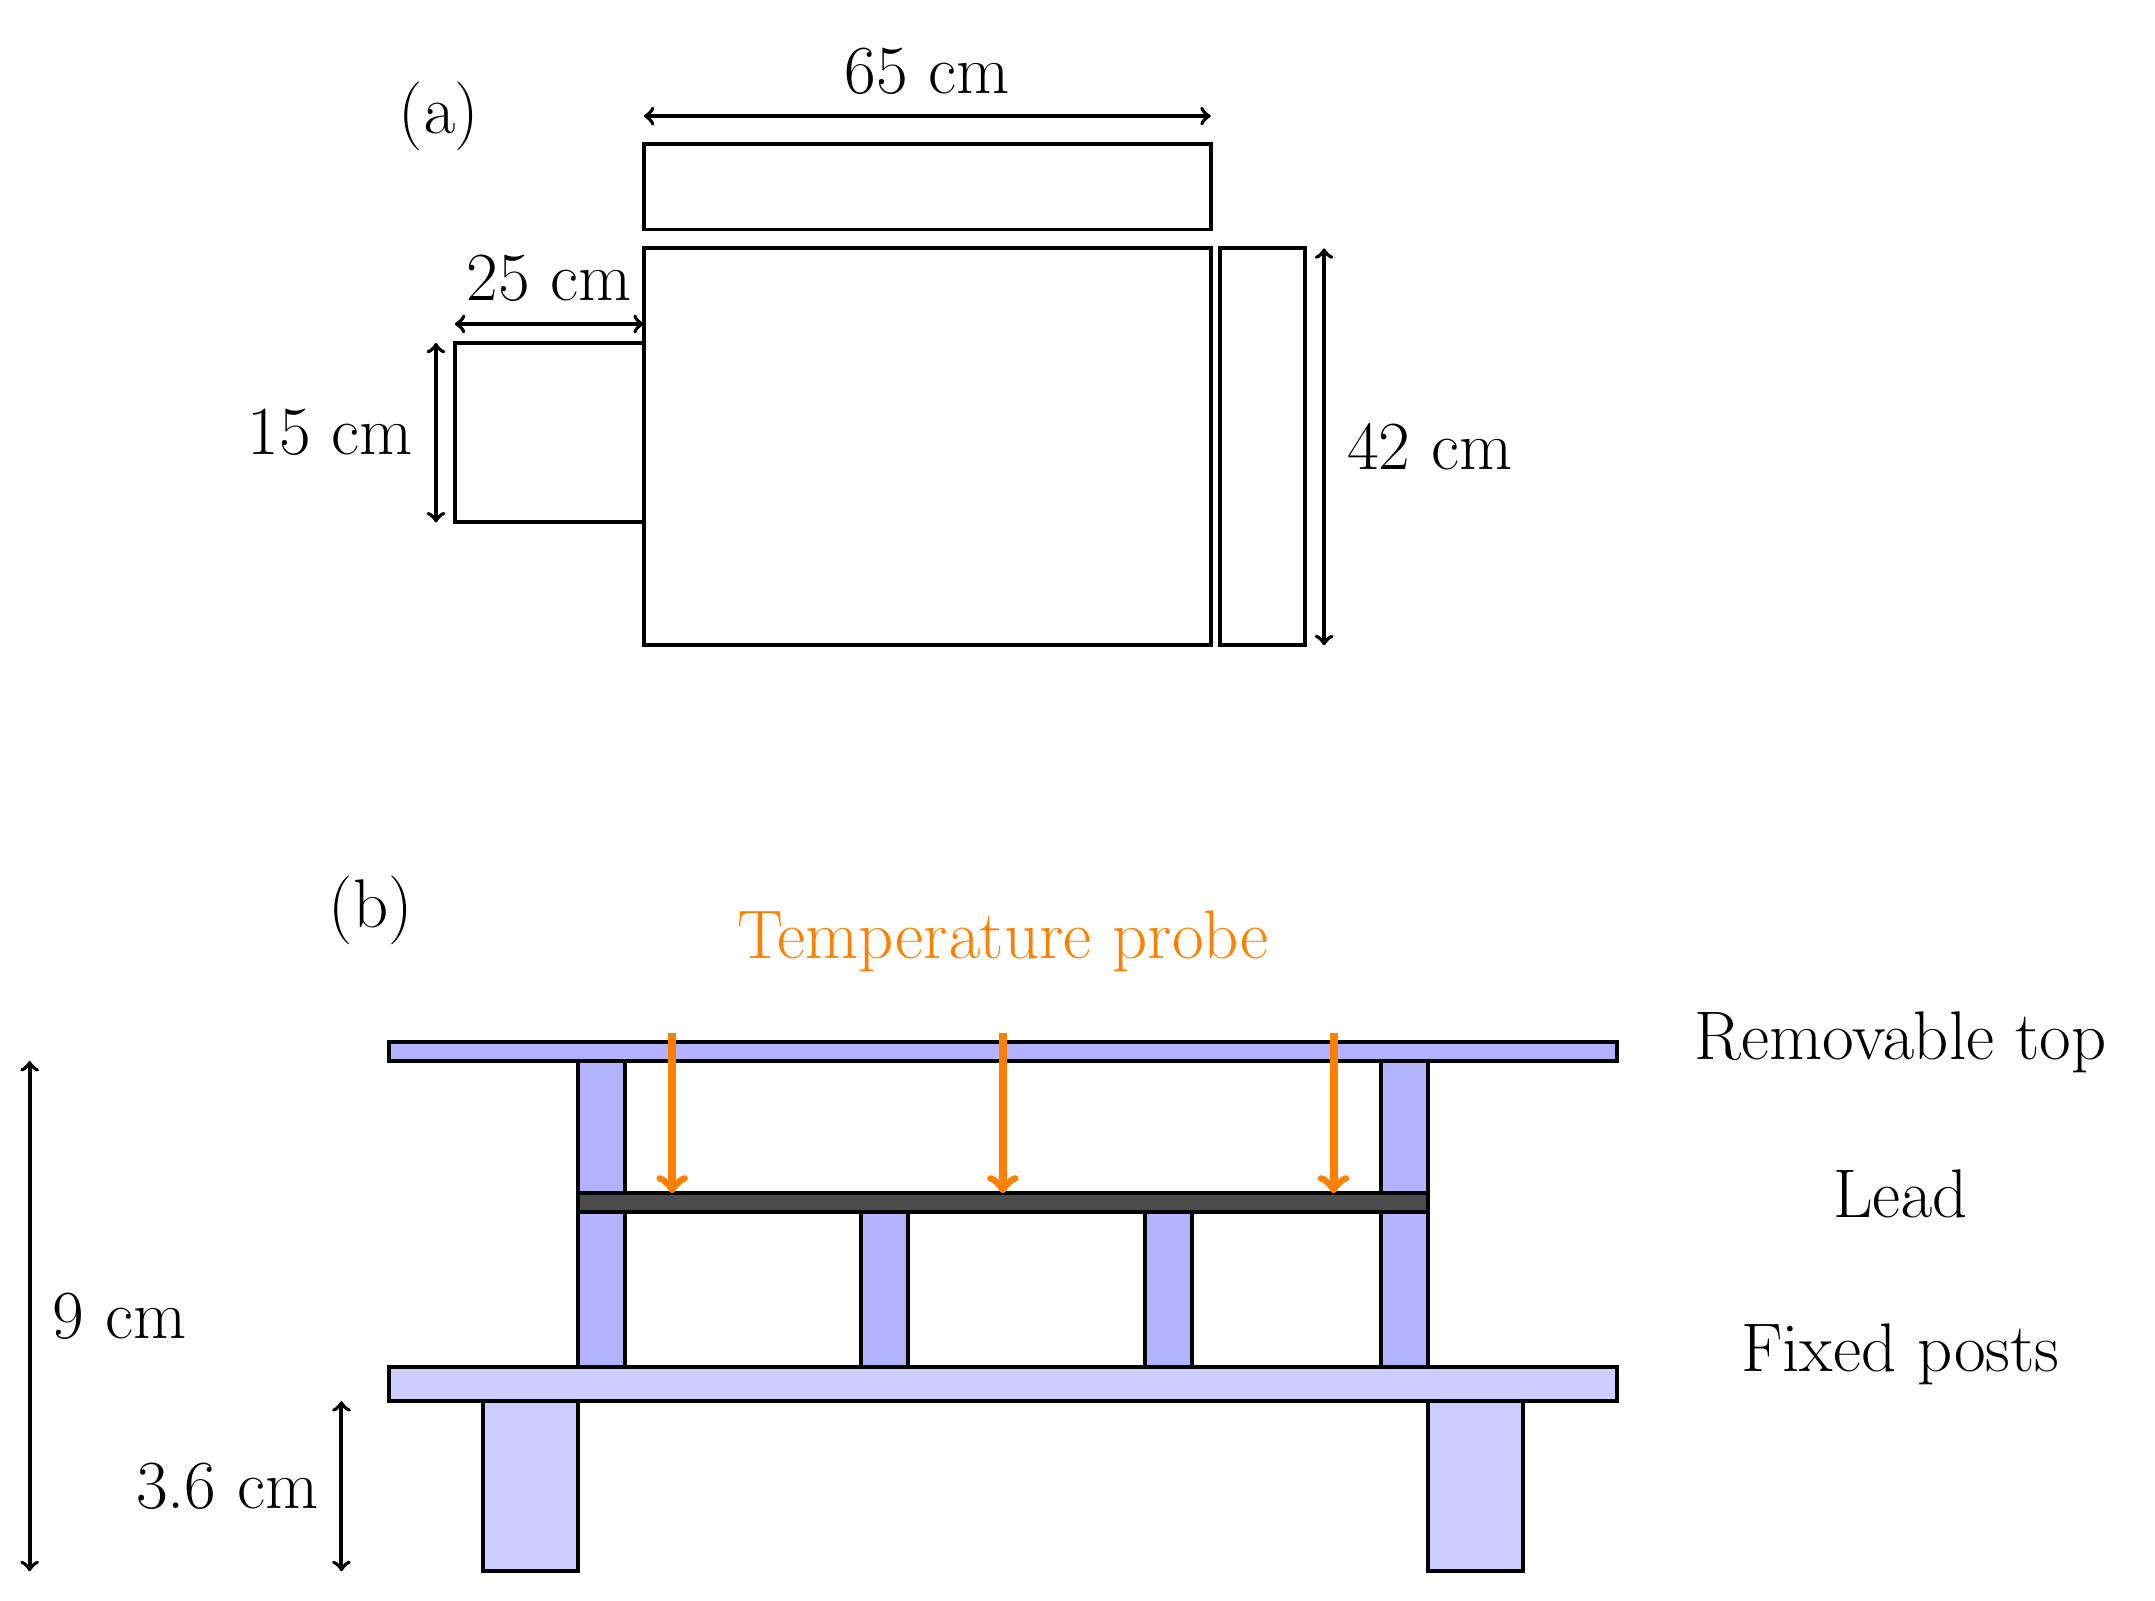
\begin{tikzpicture}[line width=0.5mm, scale=1.2]

% ----------------- (a) Top View -----------------
\node[left] at (0.5, 5.6) {(a)}; % Move label (a) to the left of the figure

% Large horizontal box (centered horizontally)
\draw[black] (2,0) rectangle (8,4.2); % Main rectangle
% Small horizontal box on top
\draw[black] (2,4.4) rectangle (8,5.3); % Slim rectangle (9cm width)
% Vertical rectangle on the right
\draw[black] (8.1,0) rectangle (9,4.2); % Vertical rectangle 42cm tall

% Square cut-out on the left
\draw[black] (0,1.3) rectangle (2,3.2); % Head as a rectangle

% Top dimensions
\draw[<->] (0,3.4) -- (2,3.4) node[midway,above] {25 cm}; % Dimension for the head
\draw[<->] (-0.2,1.3) -- (-0.2,3.2) node[midway,left] {15 cm}; % Vertical dimension for the head
\draw[<->] (9.2,0) -- (9.2,4.2) node[midway,right] {42 cm}; % Dimension for the vertical box
\draw[<->] (2,5.6) -- (8,5.6) node[midway,above] {65 cm}; % Adjusted horizontal dimension

% ----------------- (b) Side View -----------------
\begin{scope}[shift={(-.7,-8)}] % Shift the whole side view below the top view

\node[left] at (0.5, 5.2) {(b)}; % Move label (b) to the left of the figure

% Base of the table (doubled width)
\draw[black,fill=blue!20] (0,0) rectangle (13,0.36); % Base rectangle (3.6 cm tall)

% Shortened Legs below the base
\draw[black,fill=blue!20] (1,-1.8) -- (1,0) -- (2,0) -- (2,-1.8) -- cycle; % Left post
\draw[black,fill=blue!20] (11,-1.8) -- (11,0) -- (12,0) -- (12,-1.8) -- cycle; % Right post

% Fixed posts for the lead
% Two long vertical posts from base to the top
\draw[black,fill=blue!30] (2,0.36) -- (2,3.6) -- (2.5,3.6) -- (2.5,0.36) -- cycle; % Left long post
\draw[black,fill=blue!30] (10.5,0.36) -- (10.5,3.6) -- (11,3.6) -- (11,0.36) -- cycle; % Right long post

% Two short vertical posts from base to the lead
\draw[black,fill=blue!30] (5,0.36) -- (5,2) -- (5.5,2) -- (5.5,0.36) -- cycle; % Left short post
\draw[black,fill=blue!30] (8,0.36) -- (8,2) -- (8.5,2) -- (8.5,0.36) -- cycle; % Right short post

% Lead: Thin slightly longer black rectangle
\draw[black,fill=black!70] (2,2) rectangle (11,2.2); % Thin black rectangle slightly below the midpoint (2 cm)

% Top removable part (shortened distance from base)
\draw[black,fill=blue!30] (0,3.6) rectangle (13,3.8); % Removable top at 9 cm above floor

% Arrows for the temperature probes
% Left arrow
\draw[orange,thick,line width=1mm,->] (3,3.9) -- (3,2.2); 
% Center arrow
\draw[orange,thick,line width=1mm,->] (6.5,3.9) -- (6.5,2.2);
% Right arrow
\draw[orange,thick,line width=1mm,->] (10,3.9) -- (10,2.2);

% Labels for the temperature probes (moved to top)
\node[orange,align=center,above] at (6.5,4.3) {Temperature probe};

% Labels for each component
\node[align=left] at (16,3.8) {Removable top};
\node[align=left] at (16,0.5) {Fixed posts};
\node[align=left] at (16,2.2) {Lead};
%\node[align=left] at (14,0.5) {Base};
%\node[align=left] at (14,-1.5) {Legs};

% Dimension arrows for side view
\draw[<->] (-0.5,-1.8) -- (-0.5,0) node[midway,left] {3.6 cm}; % New shorter leg dimension
\draw[<->] (-3.8,-1.8) -- (-3.8,3.6) node[midway,right] {9 cm}; % Distance from floor to top

\end{scope}
\end{tikzpicture}
    \caption{Phantom design with dimensions and setup components for RF-induced heating experiments. Adapted from Aboyewa, 2021.\cite{aboyewa2021}}
    \label{fig:phantom_design}
\end{figure}

% Phantom Characterization Table (Condensed)
\begin{table}[H]
    \centering
    \renewcommand{\arraystretch}{1.1} % Slightly reduced row spacing
    \setlength{\tabcolsep}{5pt} % Reduced column spacing
    \begin{tabular}{|l|c|c|}
        \hline
        \textbf{Phantom Properties} & \textbf{ASTM F2182-11a} & \textbf{Aboyewa (2021)} \\
        \hline
        Dielectric Constant & $80 \pm 20$ & $82.1 \pm 1.4$ \\
        Electrical Conductivity (S/m) & $0.47 \pm 10\%$ & $0.47 \pm 0.04$ \\
        Thermal Conductivity (W/mK) & 0.54 & $0.850 \pm 0.007$ \\
        Density (kg/m\textsuperscript{3}) & 1000 & $1027 \pm 1\%$ \\
        \hline
        \textbf{Specific Heat Capacity (J/kg$^\circ$C)} & & \\
        New Gel (21$^\circ$C / 37$^\circ$C) & $4150 / 4190$ & $4129 \pm 47$ / $4118 \pm 48$ \\
        Old Gel (21$^\circ$C / 37$^\circ$C) & & $4207 \pm 54$ / $4166 \pm 52$ \\
        Water (21$^\circ$C / 37$^\circ$C) &  & $4168 \pm 42$ / $4151 \pm 42$ \\
        \hline
    \end{tabular}
    \caption{Results of phantom characterization as compared to ASTM standards \cite{aboyewa2021}.}
    \label{tab:phantom_characterization}
\end{table}

\begin{itemize}
    \item \textbf{Phantom Design:} Tissue-equivalent phantoms developed by Aboyewa in 2021 simulate clinical conditions, measuring RF heating under SAR values of $\sim$2 W/kg and providing a well defined methodology for simulating patient conditions and measuring RF-induced heating \cite{aboyewa2021}.
    \item \textbf{Preliminary Results:} Findings indicate leads shorter than 13 cm exhibit minimal heating under 3T MRI conditions. Orientation significantly impacts RF heating \cite{aboyewa2021}.
    %\item \textbf{Force Measurement:} Translational forces and torques were calculated using theoretical models and validated experimentally \cite{haddix2022}.
    \item \textbf{Heating Studies:} Temperature rise increases with lead length as showed on figure \ref{fig:lead_temp_rise}, this finding establishes the expected threshold for classification of leads on MRI Safety.
\end{itemize}


\begin{figure}[H]
    \centering
    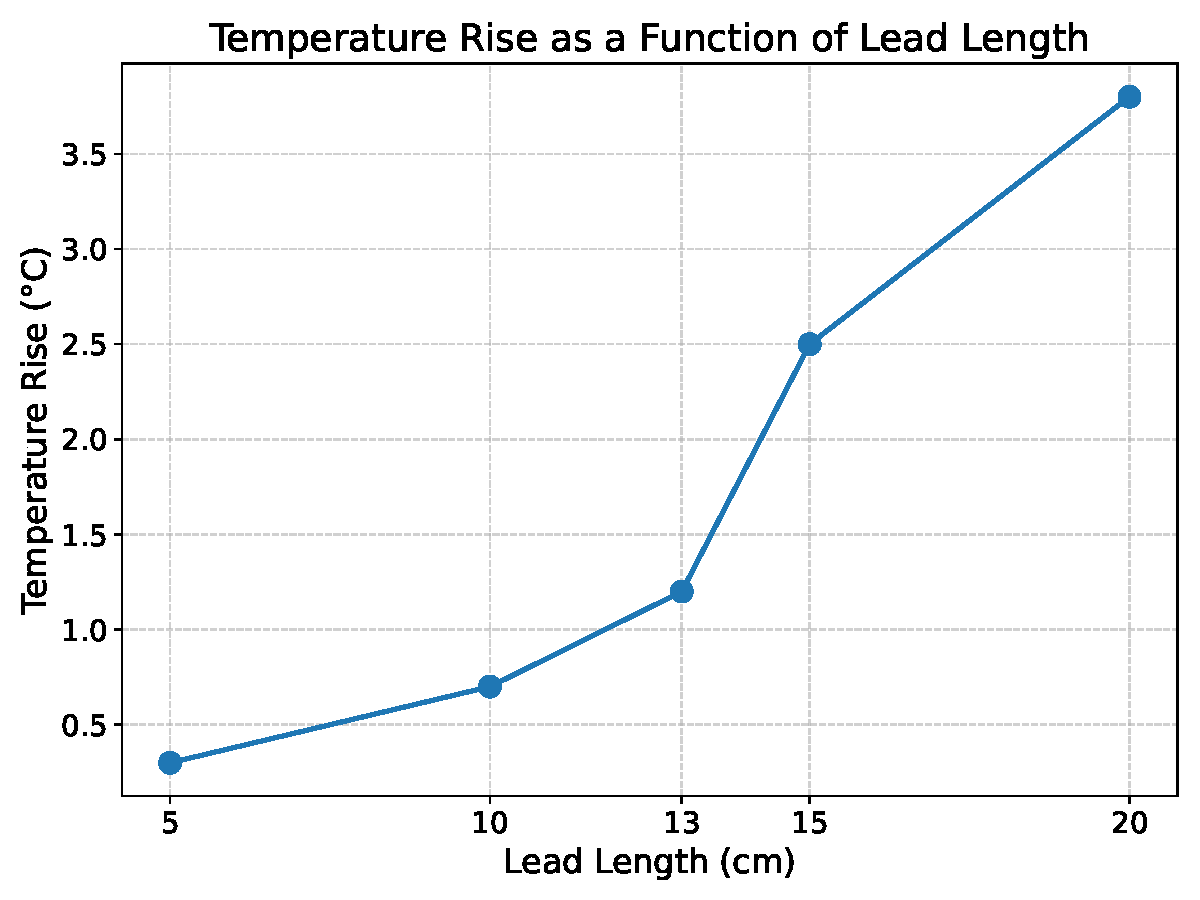
\includegraphics[width=0.6\linewidth]{FigTab.pdf} % Adjust width as needed
    \caption{Temperature rise as a function of lead length under MRI. Adapted from Aboyewa, 2021.}
    \label{fig:lead_temp_rise}
\end{figure}

\begin{quote}
Aboyewa further explored the effects of implant configuration on RF-induced heating. Figure \ref{fig:implant_orientation} illustrates the influence of implant orientation, shape, and length on maximum temperature rise.

\boldtext{Implant Configuration and RF-Induced Heating:} 
The straight configuration showed the highest temperature rise due to the antenna effect. Rotating the lead by 45$^\circ$ toward the right-side wall (TRS) or center (TC), as shown in Figure \ref{fig:implant_orientation}(b), reduced heating by more than half. An 8-fold reduction in heating was observed when the lead was bent into an arc, as shown in Figure \ref{fig:implant_orientation}(c). Although temperature rise increases with lead length \cite{aboyewa2021}, lead orientation and shape must also be considered to predict behavior in the MRI environment.  
\end{quote}

% TikZ for Top Section Adjusted and Refined
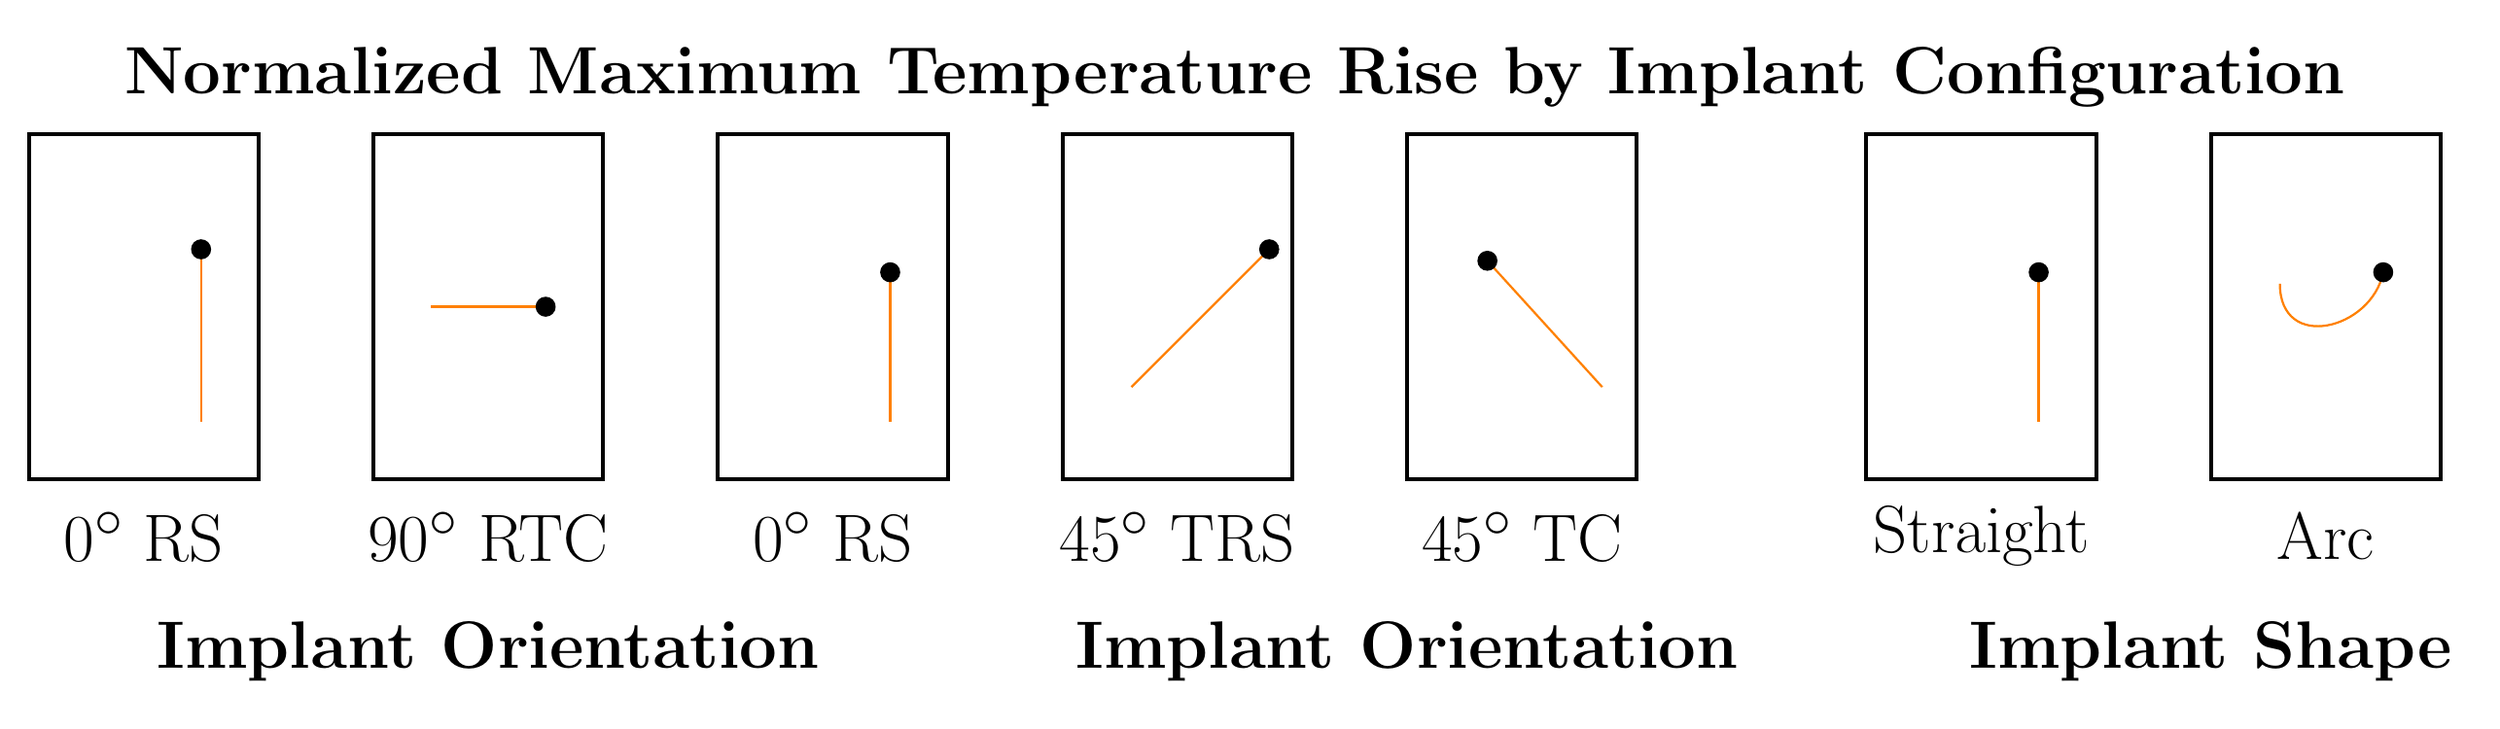
\begin{tikzpicture}[line width=0.5mm, scale=1.5]

%title
\node at (10.5, 3.5) {\textbf{Normalized Maximum Temperature Rise by Implant Configuration}};


% First Group: Implant Orientation
\node at (4, -1.5) {\textbf{Implant Orientation}};
% 0° RS
\draw[black] (0, 3) rectangle (2, 0);
\draw[orange, thick] (1.5, 2) -- (1.5, 0.5); % Adjusted position
\filldraw[black] (1.5, 2) circle (2pt);
% 90° RTC
\draw[black] (3, 3) rectangle (5, 0);
\draw[orange, thick] (3.5, 1.5) -- (4.5, 1.5); % Adjusted position
\filldraw[black] (4.5, 1.5) circle (2pt);

\node at (1, -0.5) {0$^{\circ}$ RS};
\node at (4, -0.5) {90$^{\circ}$ RTC};


% Second Group: Implant Orientation
\node at (12, -1.5) {\textbf{Implant Orientation}};
% 0° RS
\draw[black] (6, 3) rectangle (8, 0);
\draw[orange, thick] (7.5, 1.8) -- (7.5, 0.5); % Adjusted position
\filldraw[black] (7.5, 1.8) circle (2pt);
% 45° TRS
\draw[black] (9, 3) rectangle (11, 0);
\draw[orange, thick] (10.8, 2) -- (9.6, 0.8); % Refined diagonal
\filldraw[black] (10.8, 2) circle (2pt);
% 45° TC
\draw[black] (12, 3) rectangle (14, 0);
\draw[orange, thick] (12.7, 1.9) -- (13.7, 0.8); % Refined flipped diagonal
\filldraw[black] (12.7, 1.9) circle (2pt);

\node at (7, -0.5) {0$^{\circ}$ RS};
\node at (10, -0.5) {45$^{\circ}$ TRS};
\node at (13, -0.5) {45$^{\circ}$ TC};

% Third Group: Implant Shape
\node at (19, -1.5) {\textbf{Implant Shape}};
% Straight
\draw[black] (16, 3) rectangle (18, 0);
\draw[orange, thick] (17.5, 1.8) -- (17.5, 0.5); % Adjusted position
\filldraw[black] (17.5, 1.8) circle (2pt);
% Arc with V shape
\draw[black] (19, 3) rectangle (21, 0);
\draw[orange, thick] (19.6, 1.7) .. controls (19.6, 1.1) and (20.4, 1.3) .. (20.5, 1.8);
\filldraw[black] (20.5, 1.8) circle (2pt);

\node at (17, -0.5) {Straight};
\node at (20, -0.5) {Arc};

\end{tikzpicture}
\begin{figure}[H]
    \centering
    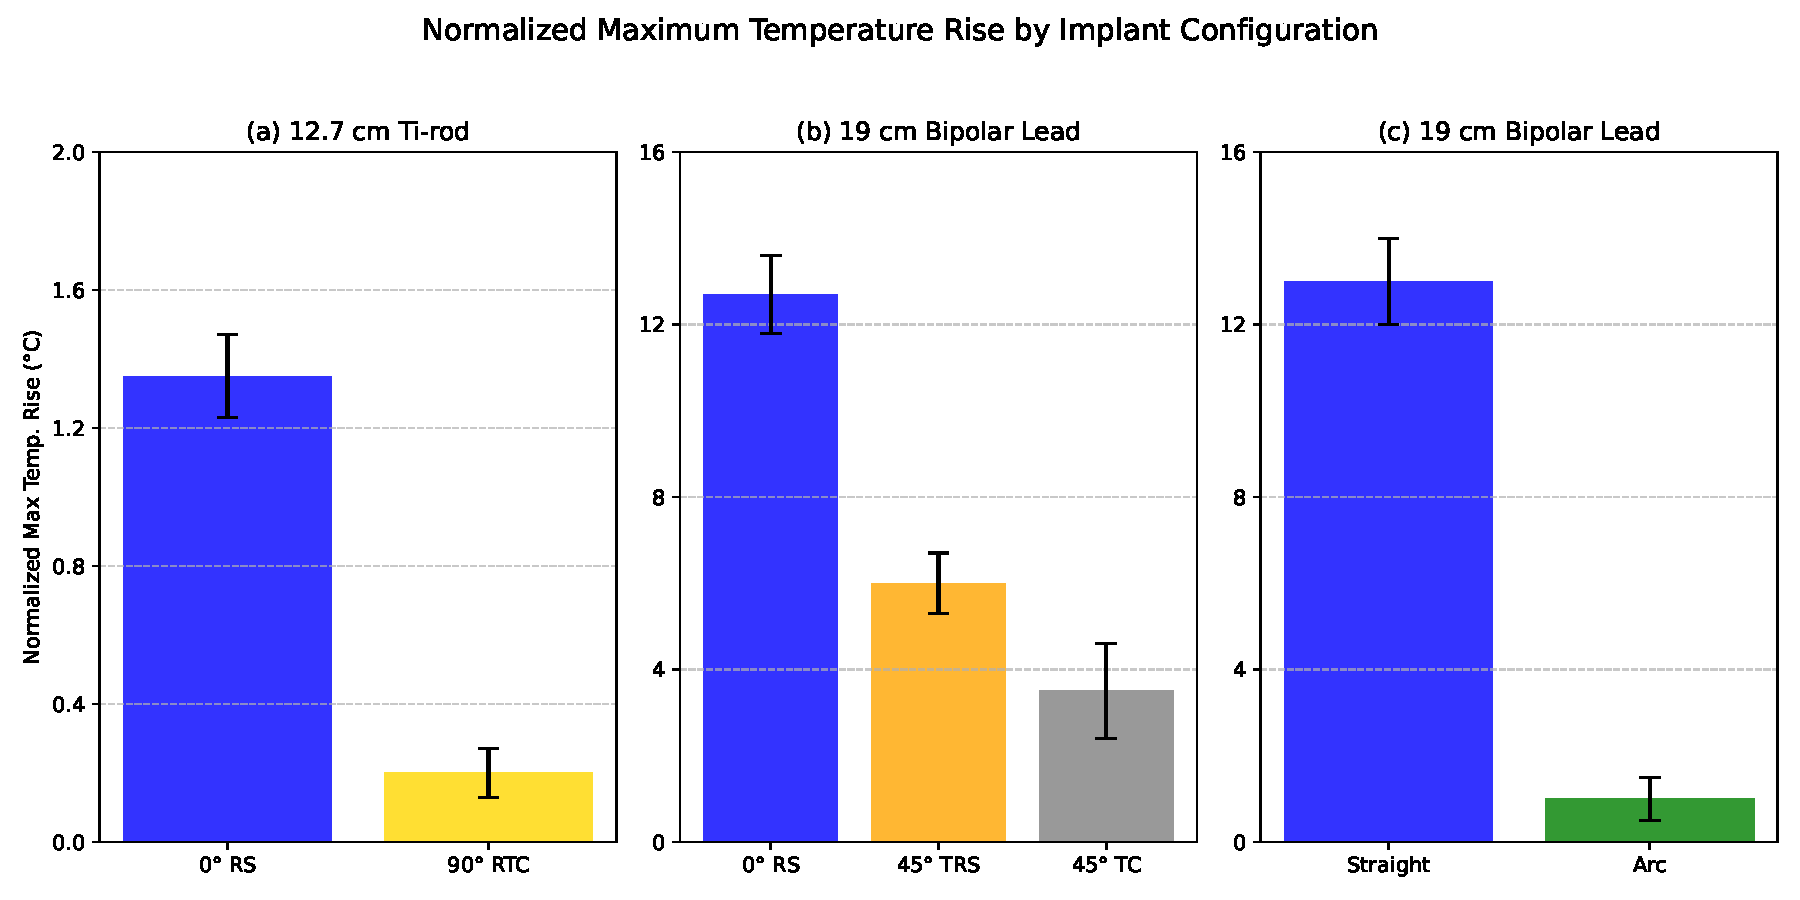
\includegraphics[width=0.9\linewidth]{Figure_4_9_Implant_Configuration_Adjusted_Y.pdf}
    \caption{Effect of implant orientation on maximum temperature rise during MRI. (a) 12.7 cm Ti-rod, (b) 19 cm Bipolar Lead, (c) 19 cm Bipolar Lead. Adapted from Aboyewa, 2021.}
    \label{fig:implant_orientation}
\end{figure}

\posterSection{Recent Advancements}
%What was learned?
\begin{itemize}
    \item \textbf{Force and Torque Studies:} The Haddix proposal outlines experiments to measure translational forces and torques, with findings suggesting that forces are typically less than 10\% of the lead's weight at the bore entrance \cite{haddix2022}.
    \item \textbf{Research Gaps:} Limited studies exist on the effects of RF-induced electrical stimulation in leads, requiring further exploration.
    \item \textbf{Safety Evidence:} Several recent studies have demonstrated the safety of MRI in patients with abandoned or epicardial leads when following specific protocols. Table \ref{tab:recent_findings} summarizes key findings from these studies.
\end{itemize}

\begin{table}[H]
    \centering
    \renewcommand{\arraystretch}{1.5}
    \setlength{\tabcolsep}{8pt}
    \begin{tabular}{|>{\raggedright\arraybackslash}p{9.5cm}|
                      >{\raggedright\arraybackslash}p{5cm}|
                      >{\raggedright\arraybackslash}p{12.5cm}|
                      >{\raggedright\arraybackslash}p{5cm}|}
        \hline
        \textbf{Study Name} & \textbf{Population} & \textbf{Key Takeaway} & \textbf{MRI Outcome} \\
        \hline
        JAMA Cardiol (2021) \cite{schaller2021} & 
        139 patients (200 MRIs) & 
        Abandoned leads no longer absolute contraindication for MRI. & 
        Safe \\
        \hline
        European Heart Journal (2021) \cite{vuorinen2021} & 
        16 patients (24 MRIs) & 
        Functional epicardial leads pose minimal risk when leads are modern (post-2000). & 
        Safe for modern devices \\
        \hline
        Magn Reson Med (2021) \cite{nguyen2021} & 
        Simulation/Phantom & 
        Abandoned leads demonstrate minimal RF heating at 1.5T/3T. & 
        Safe \\
        \hline
        Europace Meta-analysis (2024) \cite{meier2024} & 
        656 patients (21 studies) & 
        Adverse events negligible under strict protocols, justifying cautious guideline revisions. & 
        Safe \\
        \hline
    \end{tabular}
    \caption{Key findings from recent studies on MRI safety for patients with abandoned or epicardial leads.}
    \label{tab:recent_findings}
\end{table}

% Placeholder for a visual on comparative risks across devices
% \begin{figure}[H]
%    \centering
%    \includegraphics[width=0.8\linewidth]{comparative_risks_graph.pdf}
%    \caption{Placeholder: Graph comparing RF heating risks across lead types (modern vs. legacy).}
%    \label{fig:comparative_risks}
% \end{figure}

% Safety Strategies Section
\posterSection{Safety Strategies}
%What can we do?
\begin{itemize}
    \item \textbf{Technological Advances:} Improvements in MRI-conditional devices and scanning protocols have minimized risks like RF heating and device malfunction.
    \item Limiting lead lengths to reduce RF heating risks \cite{aboyewa2021} and developing MRI-specific lead configurations to minimize mechanical interactions \cite{haddix2022}.
    \item \textbf{Clinical Impact:} Updated guidelines now cautiously include patients with abandoned and epicardial leads, reducing delays in critical diagnostics.
    \item \textbf{MRI Workflow Recommendations:} In the College of cardiology an article outlines steps for preparation, monitoring, and post-scan follow-up, ensuring patient safety and device functionality for managing MRI safety protocols in patients with CIEDs depicted in Figure \ref{fig:safety_protocols}.
\end{itemize}


\begin{figure}[H]
    \centering
    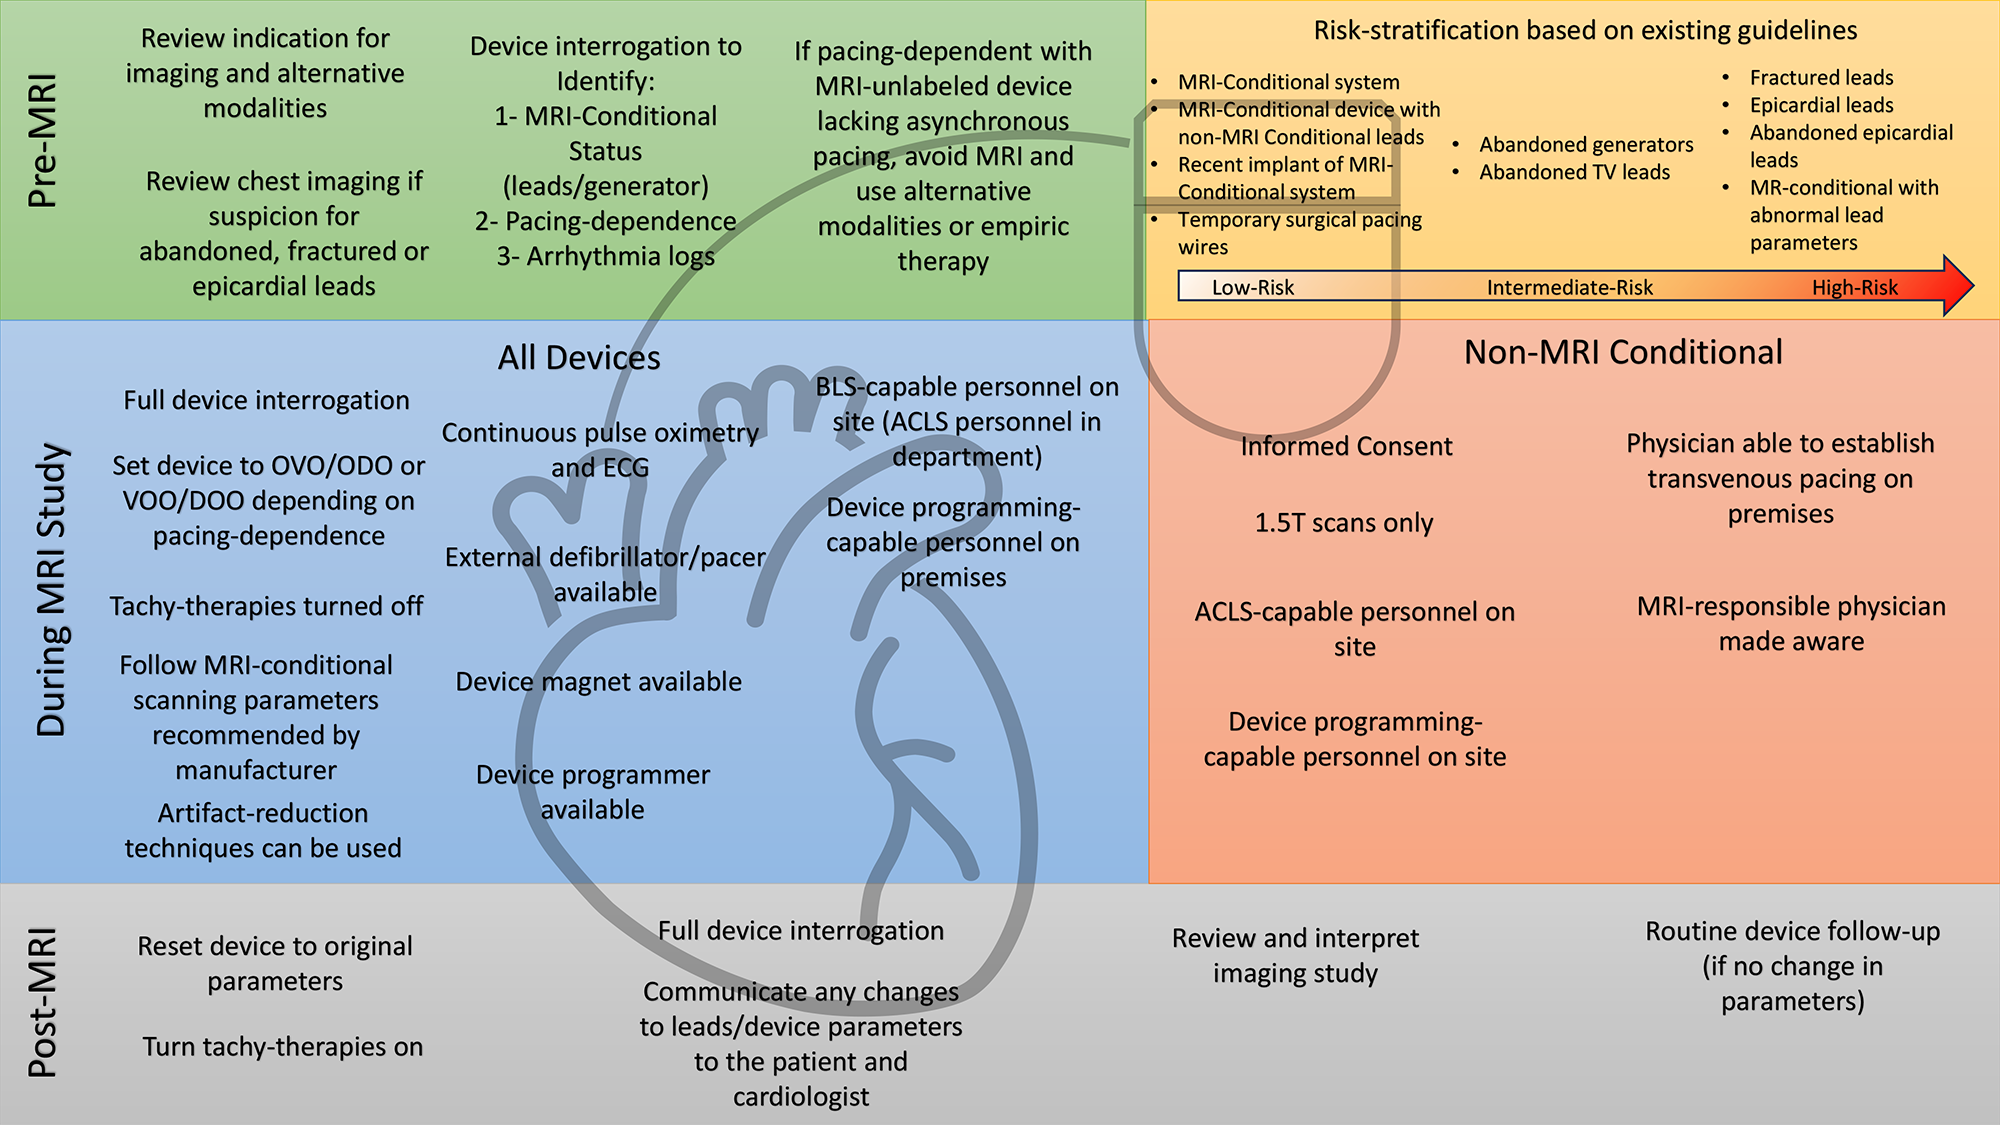
\includegraphics[width=0.8\linewidth]{IMAG-EA-Zghaib_Fig1.png}
    \caption{Comprehensive workflow for MRI safety protocols in patients with MRI-conditional and non–MRI-conditional CIEDs, covering pre-MRI preparation, during-MRI monitoring, and post-MRI follow-up.\cite{zghaib2024mri} }
    \label{fig:safety_protocols}
\end{figure}

%Acknowledgements Section
\posterSection{Acknowledgements}
This work builds upon the foundational insights provided by Dr. Nichols's proposal and Oluyemi Aboyewa’s thesis, which will serve as a basis for my forthcoming thesis research.

\vspace{-0.6in}
% References Section
%\posterSection{References}

% Suppress the default small references heading
\renewcommand{\refname}{}
% Adjust font size and spacing for references
{\fontsize{16}{23}\selectfont  % Font size: 24pt, Line spacing: 30pt
\setlength{\bibsep}{6pt}  % Slightly larger spacing between references
\bibliographystyle{unsrt}  % Choose the bibliography style
\bibliography{references}  % Point to your references.bib file
}
\end{multicols}

\end{document}
